\documentclass[11pt]{article}
\usepackage{graphicx}
\usepackage{hyperref}
\usepackage{caption}
\usepackage{amsmath}
\usepackage{mathtools}
\usepackage{physics}
\newcommand{\numpy}{{\tt numpy}}    % tt font for numpy

\topmargin -.5in
\textheight 9in
\oddsidemargin -.25in
\evensidemargin -.25in
\textwidth 7in

\begin{document}

% ========== Edit your name here
\author{Hongqing Liu, hl85}
\title{CS 498: Assignment 4: Point Cloud Segmentation}
\date{Apr 15, 2023}
\maketitle

\medskip


\section*{Submission}
In this assignment, you will implement 3D point cloud segmentation using neural networks. The starter code consists of an iPython notebook ``mp4.ipynb" which can be opened and run on Google colab. Please put together a single PDF with your answers and figures for each problem, and submit it to Gradescope (Course Code: BBX6NE). 
We recommend you add your answers to the latex template files we provided. More details on what to report are in the provided notebook. 

Reminder: Your submission should include your report pdf and filled out mp4.ipynb.

\section*{Segmentation} 

\paragraph{Question 1 (Data Loading and Augmentation)[1 pt]:}
We provide code that loads the segmentation data. In this part you will need to perform data augmentation on the loaded data within the ``ShapeNetDataset" class. In particular you should rotate the point cloud around the y-axis by a random angle, and also add some random Gaussian noise to the 3D coordinates. You should experiment with different noise levels and report the results in your pdf.

\textbf{Answer:} The codes are shown as follows, firstly I rotate the point cloud around y-axis for a random angle, then I add some noise. 
\begin{center}
    \small
    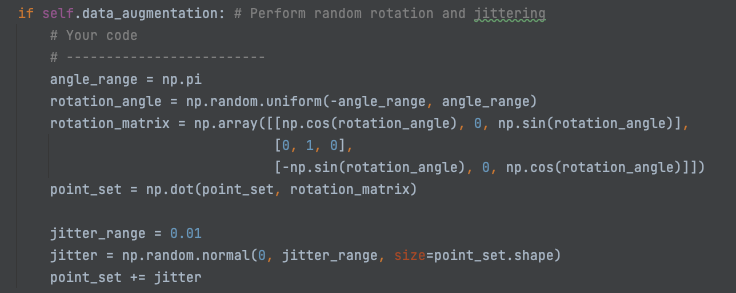
\includegraphics[width=0.3\linewidth]{fig/Q1code.png}
\end{center}
The following results are the visualization for augmentation data with noise 0.01, 0.02 and 0.05.
\begin{center}
    \small
    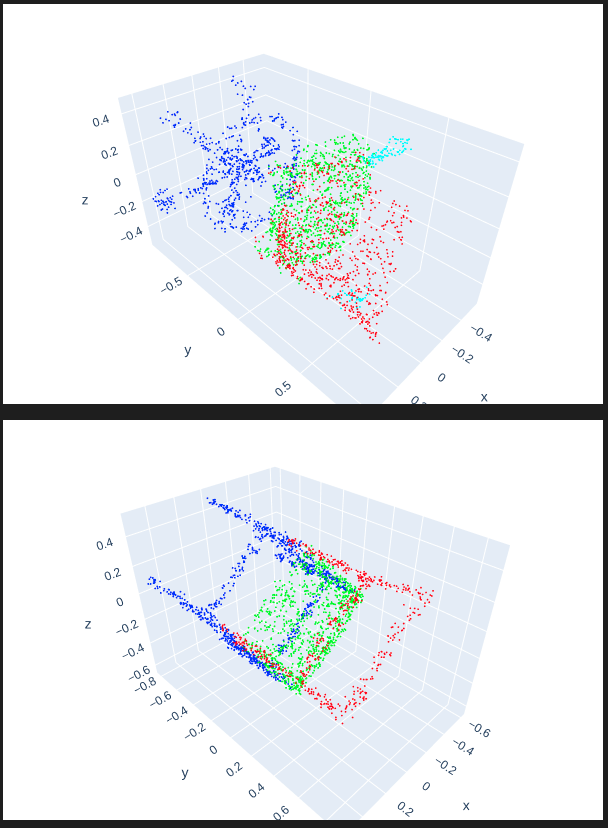
\includegraphics[width=0.3\linewidth]{fig/Q1_0.01.png}
    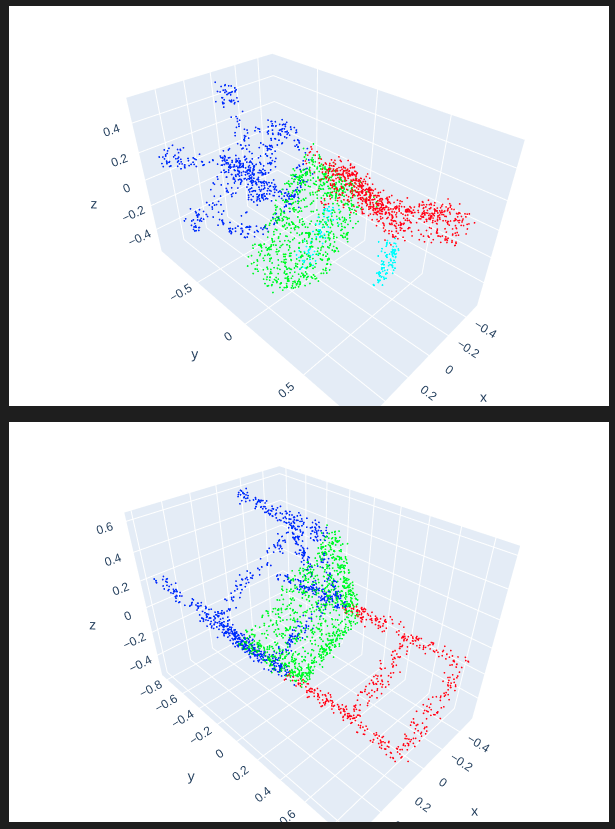
\includegraphics[width=0.3\linewidth]{fig/Q1_0.02.png}
    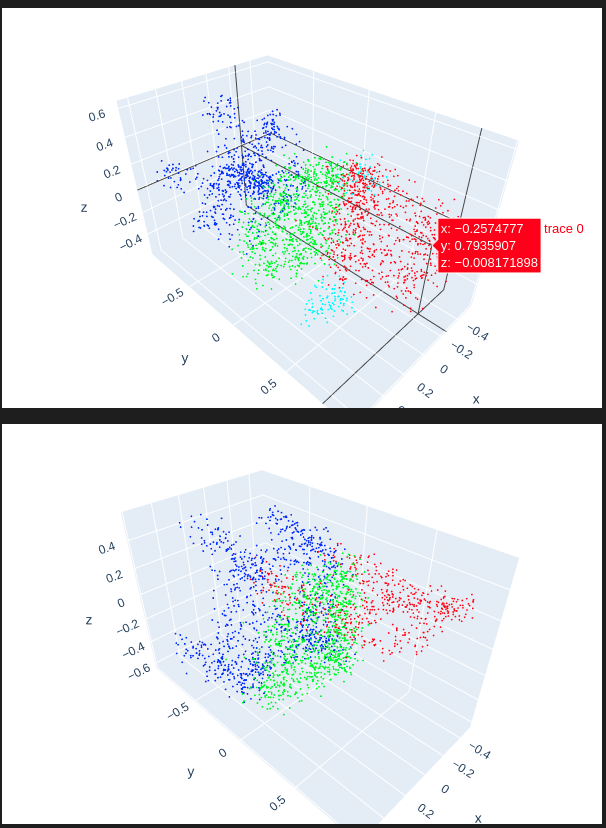
\includegraphics[width=0.3\linewidth]{fig/Q1_0.05.png}
\end{center}
It seems like that noise equal to 0.01 is the best noise for data augmentation.

\paragraph{Question 2 (Simple Baseline) [2 pts]:} 
In this part you will be modifying ``simple\_model" and ``simple\_predict" to implement a simple chair part segmentor. For each point cloud, you should segment it into thirds and predict the top third as the chair back, the middle third as the chair seat, and the bottom third as the chair legs. Determine which integer label corresponds to each class based on the visualizations from the previous question. You can run the evaluation code (from the next question) with your simple baseline and see its mean average precision which we provide - it should be around 0.54.

\textbf{Answer:} Here I sort points y value in each point cloud and put the top third as class 0 while the bottom third as class 2. The pred seg is in shape of $(16,4,2500)$. The codes are shown as follows:
\begin{center}
    \small
    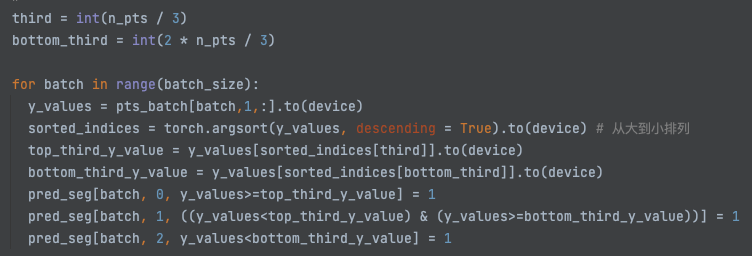
\includegraphics[width=0.3\linewidth]{fig/Q2code.png}
\end{center}
The gt seg's shape is $(16, 2500)$. The code is shown as follows:
\begin{center}
    \small
    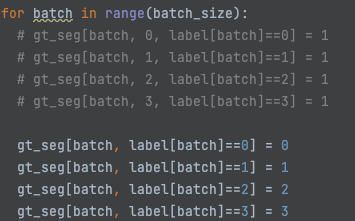
\includegraphics[width=0.3\linewidth]{fig/Q2code1.png}
\end{center}
When I write this assignment on google colab, the simple prediction function takes a lot of time, sometimes even 40 minutes. In the beginning, I think the problem is that cpu has a low speed to load and process the data, so I put the computation to gpu. Turns out that the real problem is that the pogram has to load the data from google drive every time I restart the kernel, and my internet is slow.

\paragraph{Question 3 (Evaluation Metrics) [1 pts]:}  
We must evaluate the quality of our predictions. In this part you will fill in ``compute\_confusion\_matrix". You should write code to compute the confusion matrix as well as IoU for the predicted segmentation when compared to ground truth. We provide code for visualizing the computed values as well as computing mean average precision.

\textbf{Answer:} The confusion matrix is an eye matrix with n classes dimeension while the IOU imetrics can be computed as the intersection / union. The codes and results are shown as follow, the mAP is 51.4 while the mIoU is 44.4.
\begin{center}
    \small
    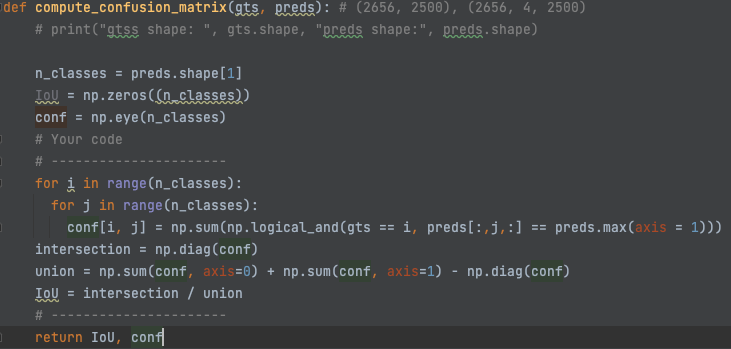
\includegraphics[width=0.3\linewidth]{fig/Q3code.png}
    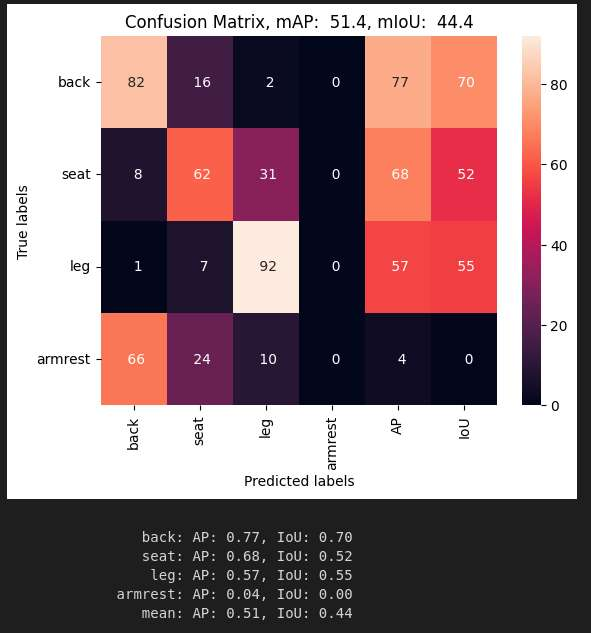
\includegraphics[width=0.3\linewidth]{fig/Q3results.jpeg}
\end{center}

\paragraph{Question 4 (Loss Function) [2 pt]:} 
To train a model we need a loss function. In this part you will fill in ``cross\_entropy\_criterion" with your implementation of the weighted cross entropy between predicted class probabilities and ground truth class labels.

\textbf{Answer:} The cross entropy loss can be written as follows:
\begin{center}
    \small
    \includegraphics*[width=0.3\linewidth]{fig/Q4code.png}
\end{center}
Firstly, I transpose the prediction matrix as (16,2500,4) and view it as (-1, 4). Here I learn how to use contiguous to make the elements stored in a contiguous block of memory.
After that, I log softmax it in its second dimension and multiply it with corresponding weights.

To choose the write log softmax value to calculate the loss, I use torch.take() function. The indices of element I choose is generated as follows.

Firstly, I reshape labels matrix into (1, 40000), each value are corresponding to the indices of the weighted log softmax we want to choose. 
For instance, if the first element is 2, it means we want to choose weighted log softmax[0][2] to calculate loss and if the second element is 1, it means we want to choose weighted log softmax[1][1], which is also weighted log softmax$[1 * 4 + 1]$ if we reshape the log softmax matrix to one row to calculate loss.

In that case, I use 

$element = torch.arange(0, labels.shape[1]).to(device)$

$labels = labels + element * predictions.shape[1]$

to choose the write labels for calculating loss.

\paragraph{Question 5 (Training Loop) [2 pt]:} 
In this part you will implement the stochastic gradient descent training loop in PyTorch, modifying ``train". We provide code to validate a trained model and a skeleton for training. 

\textbf{Answer:} The train part is pretty straight forward, firstly I put train input and train labels to gpu, secondly I zero grad the optimizer, thirdly I put the train input into the model and calculate its criterion. After that, I calculate the network's backward by $loss.backward()$ and let the optimizer train the model by $optimizer.step()$.

The validation part only calculate the loss of the model using val images and val labels, without any training. In that case, we put this part into $model.eval()$.

\paragraph{Question 6 (Model Definition and Training) [3 pt + 1 bonus point]:} 
Implement a segmentation network based on the PointNet architecture (\url{https://arxiv.org/pdf/1612.00593.pdf}, see Fig. 2). Train your models with the code you wrote for Question 5, and report results following the instructions in the notebook. 

As mentioned in the notebook, you may ignore the input-transform and feature-transform portions of PointNet and receive full credit. However, for one bonus point, you can try implementing these transforms. Details about the T-Net architecture and regularization loss can be found in the supplementary material of the paper. If you do implement the transforms, please report results with and without using them in your network. (Bonus 1 pt)

\textbf{Answer:} In this part, I will introduce the network with 3 parts. The first part is input transform and feature transform, here I utilize two models to integrate the input transform and feature transform network. 
The firt model is combined with three conv1d networks, followed by batch normalization and ReLU activation functions. The second model is combied with three linear model, followed by batch normalization and ReLU activation functions.
The different between input transform and featrue transform is that the former one has 3 input channel in the first conv layer while the second one has 64 input channel for the first conv layer.

The second part is named as point net feat, it is the part from the beginning to the concatation of global and local features. The integration primarily consists of three shared MLP models, which have been substituted with Conv1d models. t utilizes input transform before the first MLP and feature transform after the first MLP and it output the concatation of global and local feature. The output dimension is 1088.

The third part outputs per point scores. This part shows the whole network, it is combined by point net feat network and a segmentation network. The segmentation is integrated by 4 conv network, followed by batch normalization and ReLU.

The loss per epoch is shown as follows, after 20 epoches, the training loss is $0.445$ and the val loss is $0.376$.
\begin{center}
    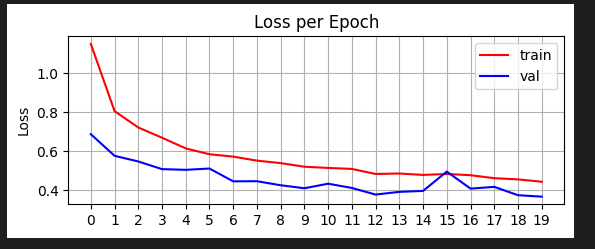
\includegraphics[width=0.3\linewidth]{fig/Q6output1.png}
\end{center}
The confusion matrix of val set is shown as follows, the mAP is $94.5$ and the mIoU is $80.8$.
\begin{center}
    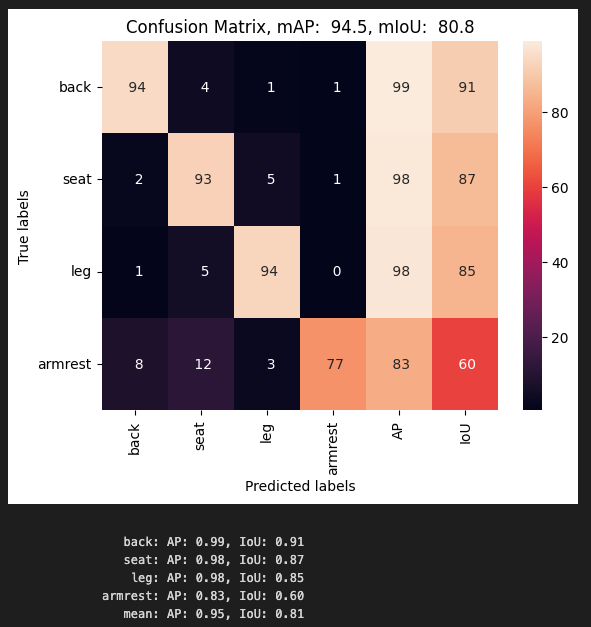
\includegraphics[width=0.3\linewidth]{fig/Q6output2.png}
\end{center}
The visulization of 3 random result in val-dataset is shown as follows:
\begin{center}
    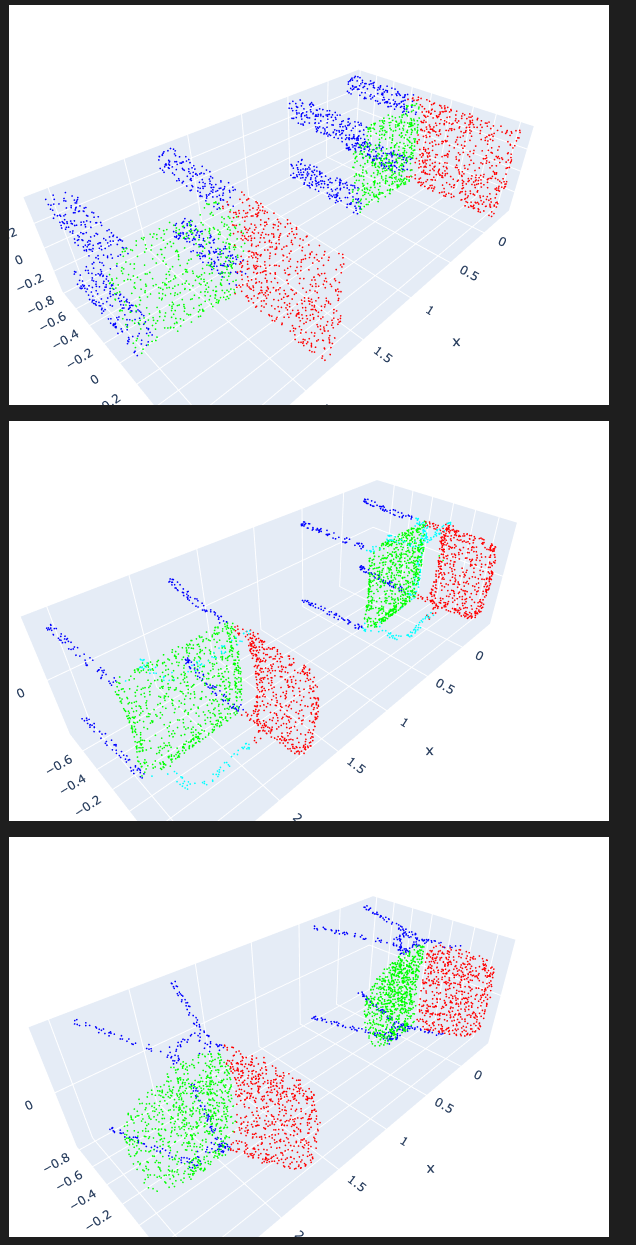
\includegraphics[width=0.3\linewidth]{fig/Q6output3.png}
\end{center}
The confusion matrix of test set is shown as follows, the mAP is $95.3$ and the mIoU is $81.1$.
\begin{center}
    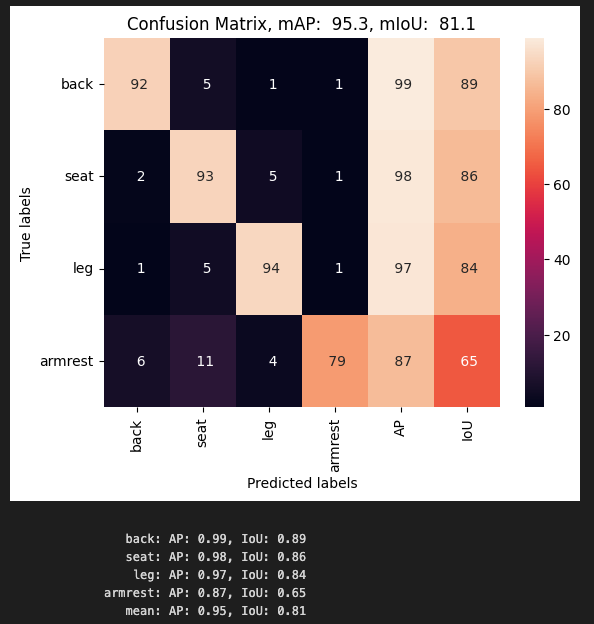
\includegraphics[width=0.3\linewidth]{fig/Q6output4.png}
\end{center}

\paragraph{Question 7 (Another Object Category) [3 pt]:} 
So far we have trained a model for chair part segmentation. However, there are many other object categories available in our dataset. Choose whichever one you like, extract the corresponding data, train a new model for that object category, and report the results. Make sure to include, training plots, final accuracy metrics, and a few visualizations of your model predictions. Also, describe what changes you made, if any, from your chair segmentation algorithm.

\textbf{Answer:} Here I use the airplane dataset, it has 4 classes. After 20 epoches of training, the results are shown as follows:
The loss per epoch is shown as follows, the training loss is $0.596$ and the val loss is $0.461$.
\begin{center}
    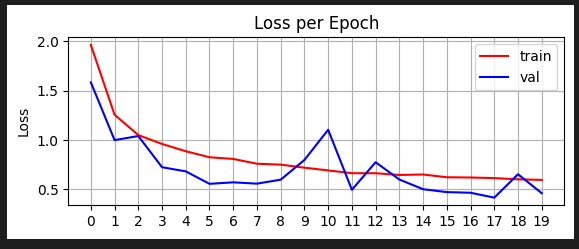
\includegraphics[width=0.3\linewidth]{fig/Q7output1.png}
\end{center}
The confusion matrix of val set is shown as follows, the mAP is $97.2$ and the mIoU is $82.8$.
\begin{center}
    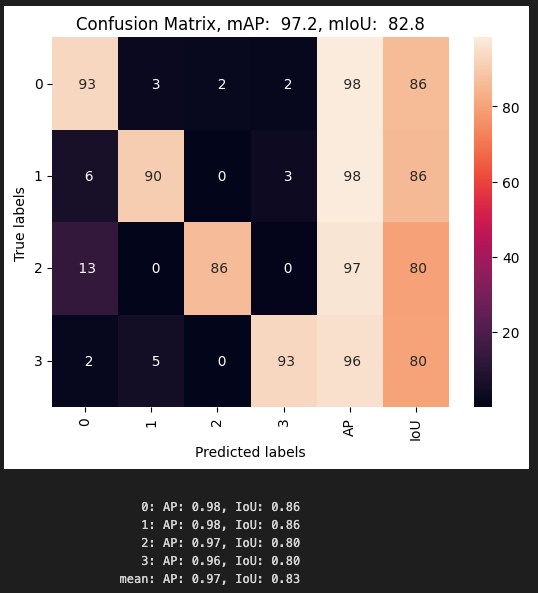
\includegraphics[width=0.3\linewidth]{fig/Q7output2.png}
\end{center}
The visulization of 3 random result in val-dataset is shown as follows:
\begin{center}
    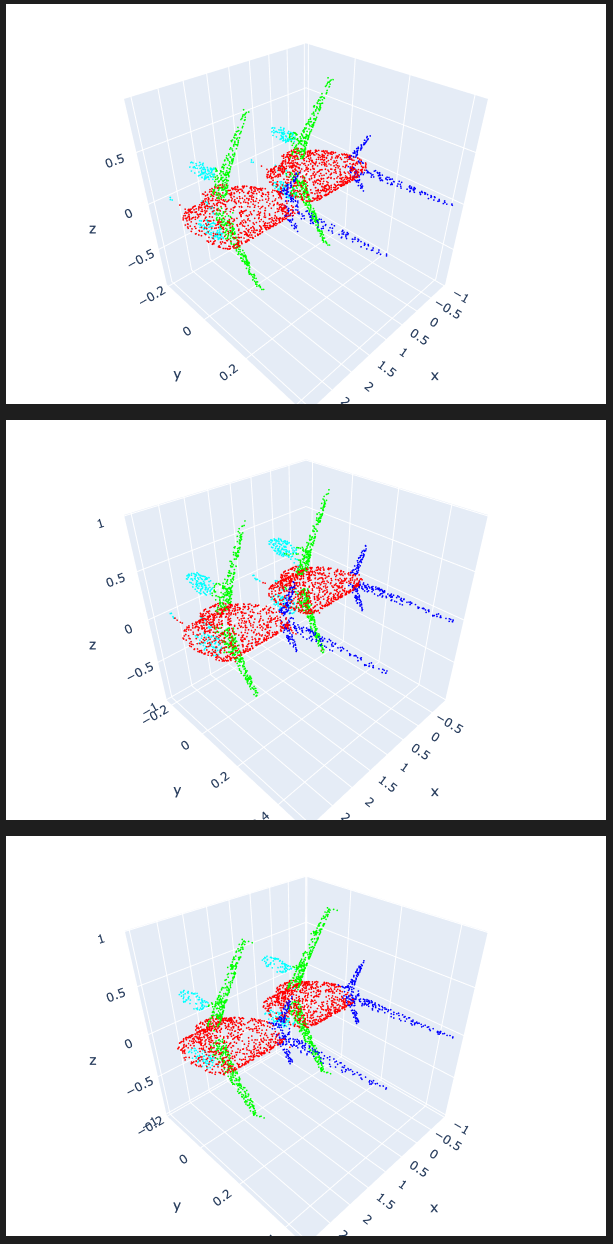
\includegraphics[width=0.3\linewidth]{fig/Q7output3.png}
\end{center}
The confusion matrix of test set is shown as follows, the mAP is $93.2$ and the mIoU is $72.9$.
\begin{center}
    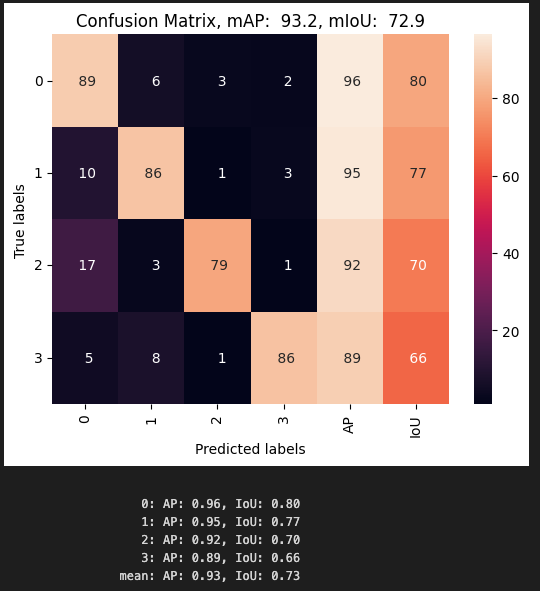
\includegraphics[width=0.3\linewidth]{fig/Q7output4.png}
\end{center}

\section*{PointNet++ (Bonus 3pt)}

PointNet achieved excellent results when it was published in 2016, but many works have built upon and improved the architecture since then. For example, PointNet++ (\url{https://arxiv.org/pdf/1706.02413.pdf}) was developed one year later and introduced hierarchical grouping to learn better features. Implement PointNet++ or another more recent point cloud segmentation architecture and evaluate its performance on our dataset.

\end{document}. 

\grid
\grid